\chapter{Modelo de integración de datos}

El mayor de los retos aplicado al análisis de variantes, es desarrollar herramientas que permitan al investigador acceder a la información fácilmente y que pueda tener una base de datos, donde pueda consultar, analizar y actualizar la información de sus experimentos \cite{Li2014}. En el campo clínico esto representa un reto aún mayor dado que se hace necesario recolectar los datos genéticos junto con los datos clínicos para poder hacer análisis más acertados y a gran escala \cite{Paila2013}. \\


Este capítulo presenta el desarrollo de un sistema para la gestión de datos para la información clínica y genómica, desde el diseño e implementación de la base de datos hasta la GUI. Este capítulo esta  organizado en diseño e implementación de datos, gestión de datos clínicos y genómicos, conclusiones. 

\section{Diseño e implementación del modelo de datos}

\subsubsection{Datos}

Se tomaron una  250 pacientes previa autorización  del laboratorio Genetix S.A.S de los cuales solo 227 contaban con consentimiento informado para utilizar la información con fines de investigación.  La información disponible, se cargo en un archivo de texto plano con la siguiente información: Edad, genéro y diagnóstico y adicionalmente para cada paciente se tenían las variantes en un archivo csv, resultado de la anotación realizada en con wAnnorvar según el pipeline implementado en el capítulo 2. 

\subsubsection{Base de datos}

Se propone el desarrollo de una base de datos relacional con información clínica y las variantes obtenidas a partir del pipeline para el llamado de variantes. Teniendo en cuenta los datos, se diseño un modelo EER que se  muestra la figura \ref{fig:t} con tablas para la gestión de variantes junto a la historia clínica. La base de datos se implemento sobre el gestor de base de datos mysql y con las herramientas de administración de Django. \\

\begin{figure}[]
	\centering
	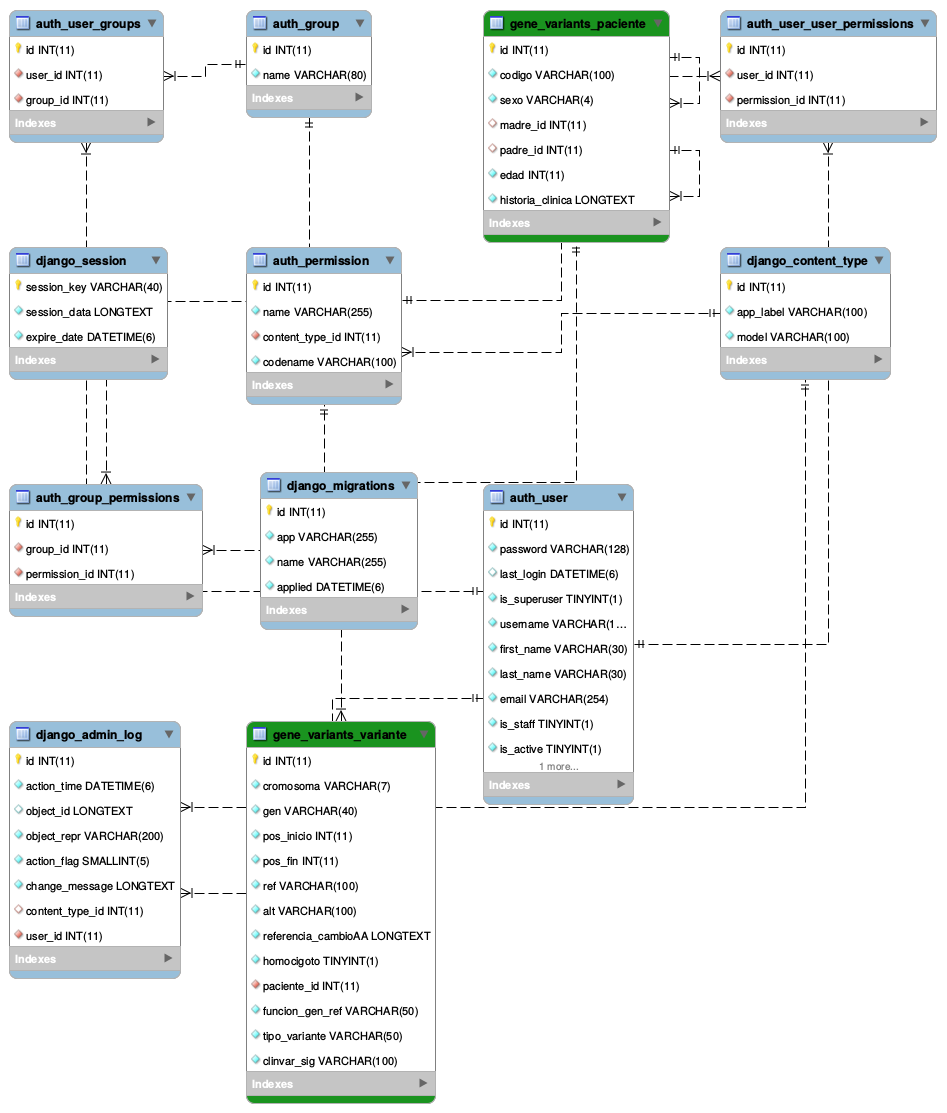
\includegraphics[width=1\textwidth]{Kap3/EER}
	\caption{Modelo entidad relación} \label{fig:t}
\end{figure}

Las tablas diseñadas para gestionar las variantes y las historias clínicas son de color verde en la figura \ref{fig:t}. La primer tabla es \textbf{gene\_variants\_paciente} descrita en el  cuadro \ref{tabla:datos} de manera detallada los datos que contiene dicha tabla. La otra tabla es \textbf{gene\_variants\_variantes} y que se describe en el cuadro \ref{tabla:datos1}. 

\begin{table}[h!]
	\begin{tabular}{|l|l|l|p{6cm}|}
		\hline
		\textit{\textbf{Campo}} & \textit{\textbf{Tamaño}} & \textit{\textbf{Tipo de datos}} & \textit{\textbf{Descripción}}             \\ \hline
		Código                  & 100                      & Carácter                       & Es el código del paciente                 \\ \hline
		Sexo                    & 4                        & Carácter                       & Indica el sexo del paciente               \\ \hline
		Madre                   & 11                       & Numérico                       & Código de madre de un paciente            \\ \hline
		Padre                   & 11                       & Númerico                       & Código de padre de un paciente            \\ \hline
		Edad                    & 11                       & Numérico                       & Edad del paciente                         \\ \hline
		Historia Clínica        & 4, 294, 967, 295            & Carácter                       & Contiene la historia clínica del paciente \\ \hline
	\end{tabular}
\caption{Diccionario de datos de la tabla gene\_variants\_paciente}
\label{tabla:datos}
\end{table}

Para la tabla \ref{tabla:datos} La edad se manejo un rango de 0-99 donde los recién nacidos o menores de un año tienen una edad de 0 y el sexo es F o M según corresponda. 

\begin{table}[h!]
	\begin{tabular}{|l|l|l|p{7cm}|}
		\hline
		\textit{\textbf{Campo}} & \textit{\textbf{Tamaño}} & \textit{\textbf{Tipo de datos}} & \textit{\textbf{Descripción}}                                         \\ \hline
		Cromosoma               & 7                        & Caracter                        & Cromosoma de la variante                                              \\ \hline
		gen                     & 40                       & Caracter                        & Nombre de los genes de las variantes                                  \\ \hline
		Pos Inicio              & 11                       & Número                          & Posicion de inicio de la variante en el genoma                        \\ \hline
		Pos Fin                 & 11                       & Número                          & Posicion de fin de la variante en el genoma                           \\ \hline
		Ref                     & 100                      & Caracter                        & Nucleótido o secuencia de referencia.                                 \\ \hline
		Alt                     & 100                      & Caracter                        & Nuecleótido o secuencia que vario.                                    \\ \hline
		Referencia              &                          & Caracter                        & Anotaciones de la variante.                                           \\ \hline
		Homocigoto              & 1                        & Binario                         & Estado alelico de la variante                                         \\ \hline
		Paciente                & 11                       & Número                          & Codigo del paciente.                                                  \\ \hline
		Funcion gen ref         & 50                       & Caracter                        & Funcion del gen                                                       \\ \hline
		Tipo de variante        & 50                       & Caracter                        & Contiene los diferentes tipos de variantes                            \\ \hline
		Clinvar sig             & 100                      & Caracter                        & Muestra el significado de la variante según la base de datos clinvar. \\ \hline
	\end{tabular}
\caption{Diccionario de datos de la tabla gene\_variants\_variantes}
\label{tabla:datos1}
\end{table}

Las variantes con su historia clínica fueron transcritas y cargadas mediante un script en bash disponible en https://github.com/jevelezse/variantesBD/blob/master/carga.bash donde se toman los archivos csv de annovar junto con los archivos de texto que tienen la información clínica del paciente en un archivo de texto plano sin formato. 

\section{Gestión de datos genómicos y clínicos}

Los resultados obtenidos fueron una aplicación con una interfaz que permite a los usuarios con poco conocimiento de  programación  analizar los datos de variantes y su resumen de la historia clínica. \\

\begin{figure}[H] 
	\centering
	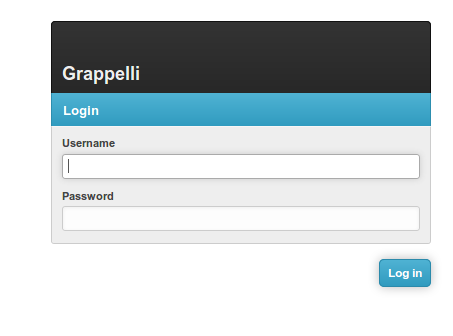
\includegraphics[width=0.4\textwidth]{Kap3/admin_django}
	\caption{Interfaz de ingreso para  administrar la base de datos. } \label{fig:admin}
\end{figure}

Inicialmente la figura\ref{fig:admin}, muestra la solicitud de usuario y contraseña para acceder a la aplicación, es diferente a la base de MySQL, pero  puede tener  una contraseña igual o diferente a la de la base de datos. \\

\begin{figure}[H] 
	\centering
	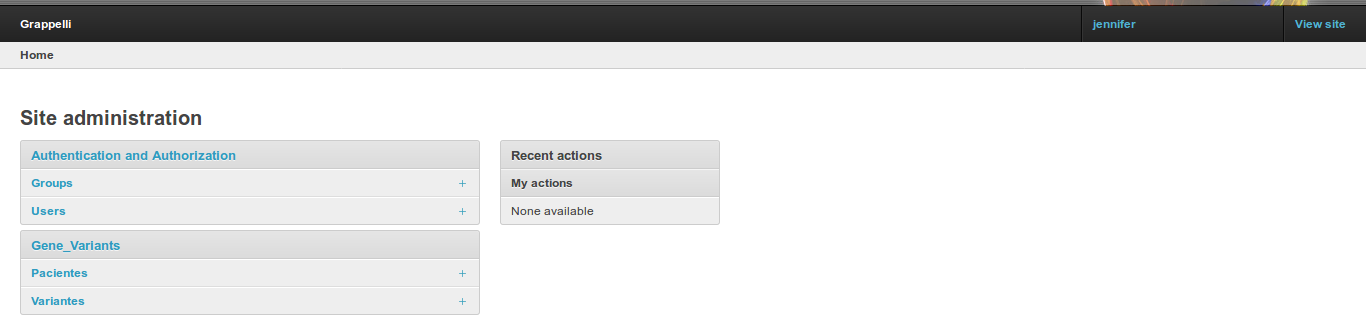
\includegraphics[width=1\textwidth]{Kap3/django_admin}
	\caption{Interfaz de administración. } \label{fig:admin2}
\end{figure}

La figura \ref{fig:admin2}, muestra el sitio de administración donde se encuentran los usuarios permitidos, las bases de datos a consultar y muestra un histórico de las actividades recientes. \\

Desde esta interfaz se puede agregar un grupo, más usuarios, pacientes y/o variantes dando click en el signo más sin necesidad de hacer la carga directa a MySQL ya que Django se encarga de hacer la carga, lo que permite actualizar los cambios que se reporten para la variante, por ejemplo variantes que por su alta frecuencia poblacional dejan de ser variantes y se convierten en referencias.\\

\begin{figure}[h] 
	\centering
	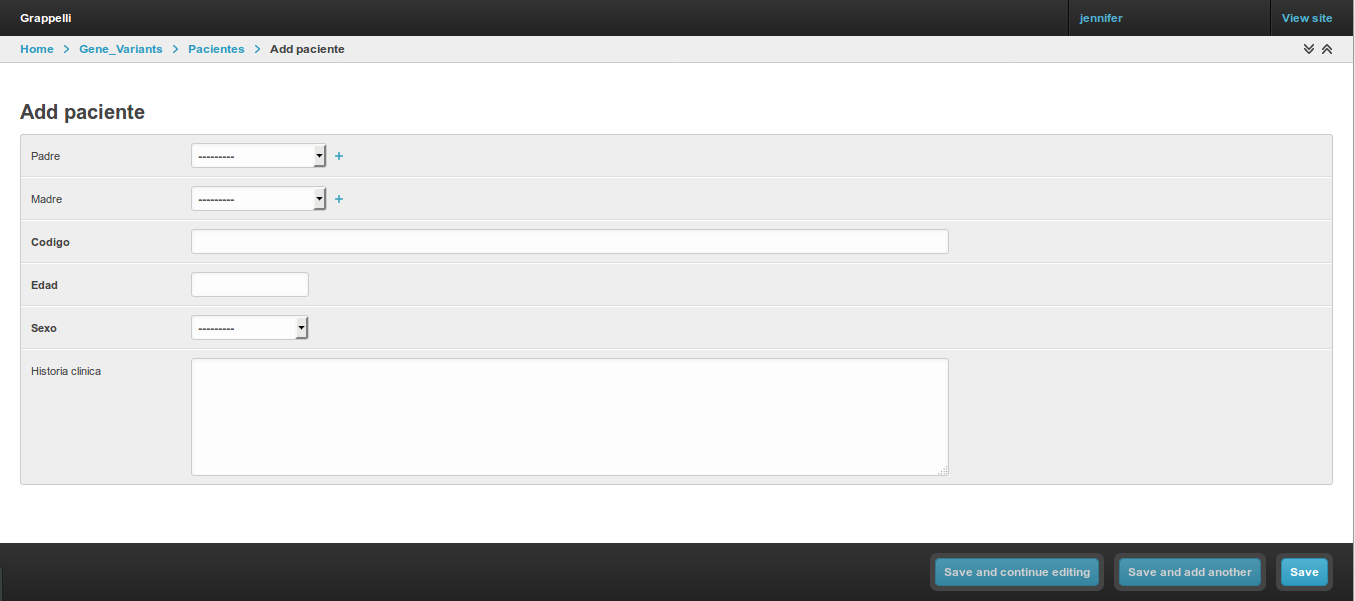
\includegraphics[width=1\textwidth]{Kap3/ingresar_paciente}
	\caption{Ingreso de pacientes.} \label{fig:pacientes}
\end{figure}

En la figura \ref{fig:pacientes} se muestra el formulario para ingresar una nueva historia o de modificar una historia clínica de un paciente de manera manual. \\

\begin{figure}[h] 
	\centering
	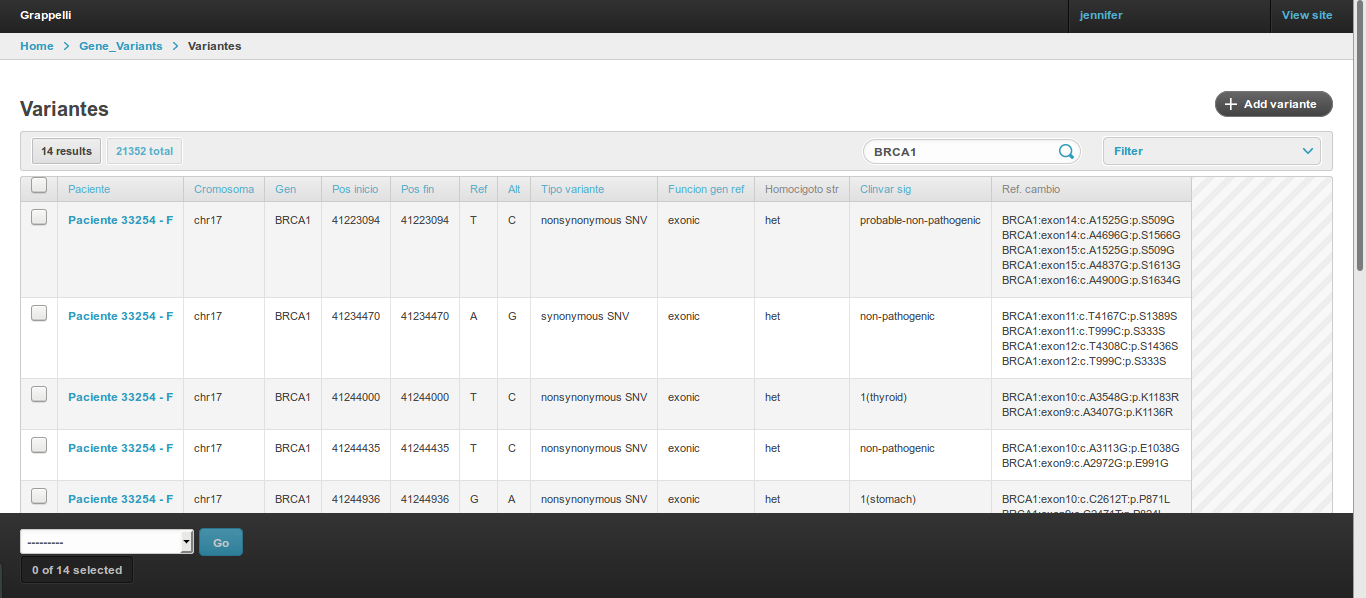
\includegraphics[width=1\textwidth]{Kap3/consulta}
	\caption{Consulta a variantes} \label{fig:consulta}
\end{figure}


La figura \ref{fig:consulta} muestra una consulta de las variantes que se tienen cargadas en la base de datos para el gen BRCA1, donde nos muestra una consulta de las variantes con su anotación  filtrada mediante un script de python antes de cargar las anotaciones de la tabla obtenida por annovar para cada paciente. Desde esta misma interfaz se puede hacer consultas de pacientes que se deben eliminar, en la parte inferior se encuentra la opción. \\

Si se desea hacer modificaciones a los datos del paciente también es posible hacerlo desde esta misma interfaz seleccionando el código del paciente, que lleva a la tabla de genes\_varante\_paciente que contiene el formulario de la historia clínica con los datos cargados para ser modificados. \\

La importancia de gestión aplicada al manejo de datos clínicos y de información genética es de vital importancia dado que existen miles de anotaciones que requieren de scripts para cargarlos las anotaciones y como es este caso el historial clínico del paciente \cite{Paila2013}.\\

La aplicación desarrollada para crear y gestionar una base de datos aplicada una bioinformática con aplicaciones a la medicina, es necesario que la base de datos provea las consultas para soportar las decisiones sobre un paciente en especifico teniendo en cuenta sus datos, la relación con datos de otros pacientes y los datos de exomas, además de los datos relacionados con los familiares en caso de que se encuentren estos datos. Mostrando que es posible realizar una integración adecuada de los datos bioinformáticos y clínicos utilizando bases de datos relacionales, con una buena respuesta en las consultas. \cite{Sujansky2001}. 

\section{Conclusión}

La utilización de aplicaciones en Django permite que un bioinformático diseñe e implementar bases de datos aplicadas al diagnóstico clínico, donde se puede guardar y gestionar toda la información obtenida de un paciente, lo que permite hacer análisis a profesionales Médicos y biólogos fácilmente. Una vez ha sido implementa la base de datos también es posible aplicar técnicas de minería de datos para optimizar los análisis de la información. \\

\section*{Resumen}

En este capítulo se presentó el proceso de diseñar e implementar un sistema de información para la gestión de datos clínicos y genómicos, dada la importancia de tener toda la información integrada para hacer futuros análisis. Se utilizó la herramienta de Django como gestor de la base de datos, se transcribió las información clínica y se cargaron las variantes obtenidas para cada paciente, como resultado se generó un sistema de información que permite realizar consultas de variantes con las características clínicas de los pacientes.   